

\chapter{Electron, Muon, and Jet Reconstruction}

\section{Electron Reconstruction}

Electrons are reconstructed from the tracks they form in the silicon tracker and from their energy which is deposited in the ECAL. An electron passing the silicon tracker looses energy through ionization and the emission of a photon (this process is called bremsstrahlung). This energy loss has to be taken into account.  Electron reconstruction needs to join both the tracks in the tracker and the energy deposit in the ECAL while successfully identifying the particle as an electron.  All this must happen while being careful not to identify other charged particles (like pions) as electrons. A particle incorrectly identified as an electron is called a fake electron. To take this and other problems into account, there are two different clustering algorithms that are used~\cite{Meschi:687345}. 

The energy that is collected in the calorimeter is grouped together into super-clusters. This is done along the $\phi$ direction by taking the most energetic cluster and collecting the other nearby clusters together. Once a super-cluster is created, a minimum of two hits is needed in the pixel detector in order to start the electron trajectory reconstruction. Using the trajectory, momentum, and the loose geometrical matching with the super-cluster, the tracks are matched to the appropriate super-cluster. There are four different electron classes that are corrected in different ways for bremsstrahlung and other effects.  The four types are as listed~\cite{Baffioni:934070}:

\begin{itemize}
\item
  Golden electrons. This class represents electrons least affected by radiation emission, with a reconstructed track well matching the supercluster and a well behaved supercluster pattern. 
\item
  Big Brem electrons. This class contains electrons with a good match between the energy calculated in the supercluster algorithms and the momentum recorded coming in but the supercluster does not directly match with the reconstructed track.  Also, there must be no energy loss effects from secondary photon conversion. Electrons for which all the bremsstrahlung is radiated in a single step can fall in this category.
\item
  Narrow electrons. In this intermediate class, electrons have a large bremsstrahlung fraction but not has high as Big Brem electrons.  There is a well behaved supercluster (i.e. the bremsstrahlung photons are merged inside a single cluster), but like Big Brem, it doesn't have a clean match between the tracks and the supercluster.
\item
  Showering electrons. This class contains electrons which failed to enter any of the above classes. It includes electron supercluster patterns involving one or several identified bremsstrahlung sub-cluster(s), or cases where a bad energy-momentum $E/p$ matching is observed. This is very likely in cases of secondary conversion of some early radiated bremsstrahlung for electrons having radiated a large fraction of their initial energy.
\end{itemize}

Once the electrons are corrected, the Gaussian-sum filter (GSF) algorithm for electron reconstruction is used to model the bremsstrahlung energy loss distribution by a Gaussian mixture rather than by a single Gaussian ~\cite{GSF_at_CMS}. Further cuts can be done as part of an analysis or for pre-selection to reduce fake electrons.

\section{Muon Reconstruction}

In the CMS detector muon tracks are reconstructed both in the tracker and in the muon chambers.  The muons must transverse a large amount of material before they reach the muon chambers, which lowers the resolution because of the scattering that has happened. This places a great importance on the tracker measurements both for the fine resolution and the intense magnetic field. 

First the muon tracks are reconstructed from the muon chambers. Then in a two step process these tracks from the muon chambers  are linked to the corresponding tracks found in the tracker.  First a set of tracks that match the momentum and direction of the muon chamber tracks is found.  After that a matching algorithm is applied using kinematics and angular variables to find the most accurate tracker/muon chamber track pair.
% Figure~\ref{fig:muon_pandolfi}~\cite{Pandolfi_thesis}

\begin{figure}[htb]
\centering
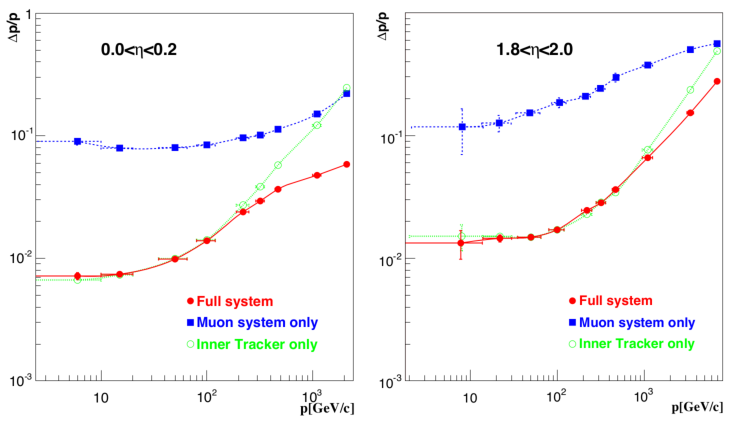
\includegraphics[width=0.69\textwidth]{Reconstruction/muon_Pandolfi.pdf}
\caption{Muon momentum resolution when using the muon spectrometers only (blue), the tracker only (green), and the full system (red): barrel ($|\eta| < $0.2) results are shown on the left, end-caps (1.8 $< |\eta| <$ 2.0) on the right.~\cite{Pandolfi_thesis}}
\label{fig:muon_pandolfi}
\end{figure}

A muon candidate made from the muon chambers and tracker information is called a global muon. If a global muon cannot be reconstructed, then using only the tracker information a tracker muon is created.  Similarly, if only a track from the muon systems is found it is reconstructed to be a stand alone muon. The High-Level Trigger uses additional criteria for a selection like isolation and momentum to create datasets for later analysis.

\section{Jet Reconstruction}

At proton colliders the reactions are primarily from the interaction of partons, which is the name given to the constituents that make up a hadron. Hadronization gives rise to columns of particles that we call jets. Jets are difficult for both theorists and experimental physicists because they are composite objects that cannot be specifically defined.  The jet reconstruction that is used is based on how particle candidates cluster using the particle flow (PF) algorithms which are described below.  This composite nature causes the detector response to vary jet to jet. This becomes a problem for the determination of the jet's energy and necessitates careful calibrations.

Light particles make up of the bulk of hadronization.  The typical breakdown of a jets energy is as follows:
\begin{itemize}
 \item
about 65\% of a jet energy is carried by charged particles, predominantly
charged pions and kaons;
\item
 20\% is converted into high-energy photons, mainly from the electromagnetic
decay of neutral mesons such as $\pi$'s and $\eta$'s;
\item
 the remaining 15\% is stored in long-lived neutral hadrons, mainly neutral
kaons, neutrons, and $\Lambda$ baryons.~\cite{Pandolfi_thesis}
\end{itemize}

With only 20\% of the jet energy being purely electromagnetic, the remaining measurements are taken through the hadronic calorimeter which leads to additional energy measurement difficulties.

The clustering of the particles that make up the jets is done with the anti-$K_t$ algorithm.  This algorithm is described in the following section. 

We first define $d_{ij}$ and $d_{iB}$~\cite{1126-6708-2008-04-063}:
\begin{equation}
d_{ij} = \min(k_{ti}^{2p}, k_{tj}^{2p}) \frac{\Delta_{ij}^2}{R^2}\,,\\
d_{iB} = k_{ti}^{2p}\,
\end{equation}

$\Delta_{ij}^2 = (y_i-y_j)^2 + (\phi_i - \phi_j)^2$ and $k_{ti}$, $y_i$ and $\phi_i$ are respectively the transverse momentum, rapidity and azimuth of particle $i$. First we find the minimum of all the distances $d_{ij}$ and $d_{iB}$. If the minimum is one of the $d_{iB}$ then it is called a jet and if it is a $d_{ij}$ we combine $i$ and $j$ into a new particle by summing over the momentum.  We continue to do this until we only have jets.

One of the benefits of this algorithm is that the distance parameter R only allows particles to be merged into jets of that specific radius or smaller.  This also results in conical jets that have radius equal to or smaller than this distance parameter. This can be seen in figure~\ref{fig:anti_atk}~\cite{1126-6708-2008-04-063}. In this analysis the R value is 0.5.

\begin{figure}

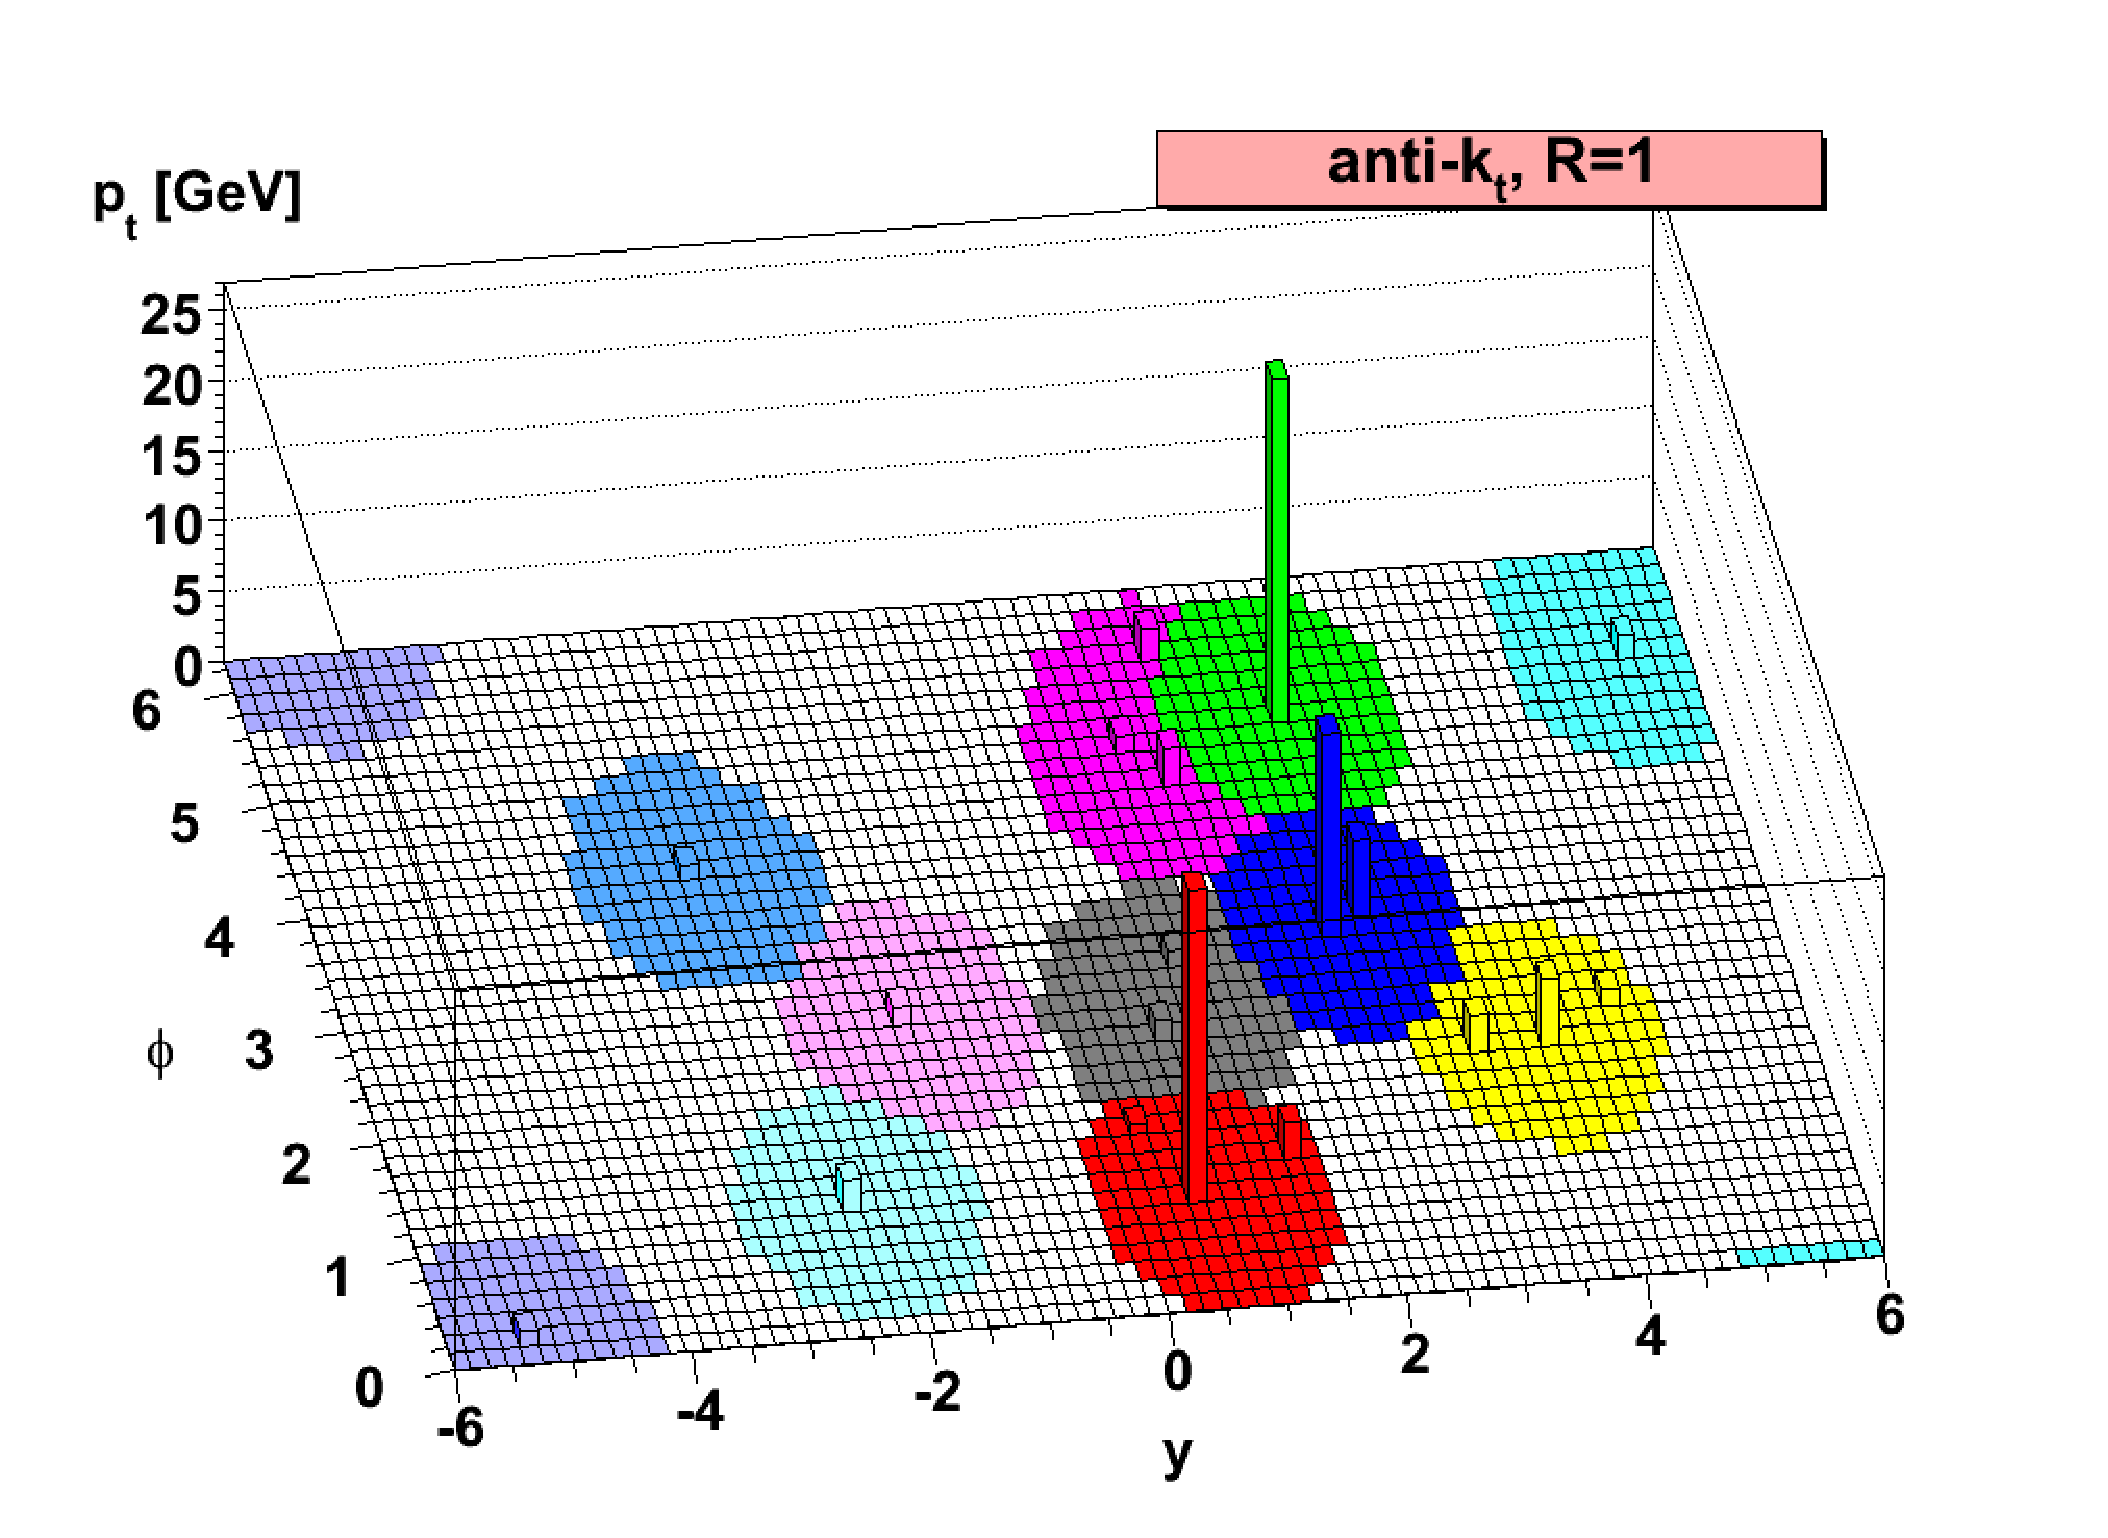
\includegraphics[width=0.79\textwidth]{Reconstruction/herwig-parton-level-ev-antikt-R1-ghosted4root.eps}
\centering
\caption{A sample parton-level event (generated with
    Herwig~\cite{Herwig}), together with many random soft ``ghosts'',
    clustered with the anti-$k_t$ algorithm, illustrating the
    ``active'' catchment areas of the resulting hard jets. This shows the cylindrical jets all with radius of R=1 or less.~\cite{1126-6708-2008-04-063}}
\label{fig:anti_atk}
\end{figure}

\section{Particle Flow Reconstruction}

At CMS particle-flow event reconstruction tries to reconstruct and identify all stable particles in the events.  This includes all the electrons, muons, charged and neutral hadrons, and photons.  It also uses information from all the sub-detectors like the tracker, both calorimeters, muon chambers, etc. After detection these particles are used as if they were Monte Carlo generated events to build the jets, MET, taus, lepton isolation, tag b-jets, and more~\cite{particleflow}.

This is possible because the CMS detector has such a large silicon tracker fully immersed in the magnetic field and the large pseudo-rapidity range. This allows particle detection for particles that have a transverse momenta as low as 150 MeV.  As previously mentioned, jet energy is only 15\% in the hadronic calorimeter. Figure~\ref{fig:jet_energy_components}~\cite{Pandolfi_thesis} shows the energy fractions as a function of pseudorapidity for the reconstruct jets on MC simulation.  


\begin{figure}
\begin{center}
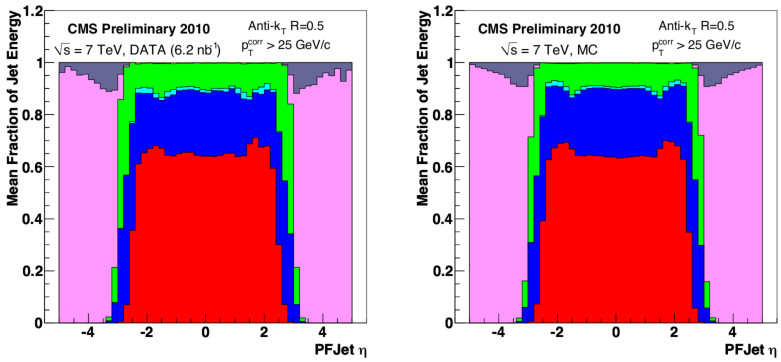
\includegraphics[width=0.99\textwidth]{Reconstruction/Pandolfi_jetenergy.pdf}
\caption{Reconstructed jet energy fractions as a function of jet pseudo-rapidity. In the central region, bottom to top: charged hadrons (red), photons (blue), electrons (cyan), neutral hadrons (green). In the forward region: HF hadrons (pink), HF electromagnetic particles (gray).~\cite{Pandolfi_thesis}}
\label{fig:jet_energy_components}
\end{center}
\end{figure}

The Particle Flow algorithm works as follows. The hits in each part of the detector are independently reconstructed and formed into blocks.  These include tracks in the tracker and calorimeter energy deposit clusters. After the blocks are formed a linking algorithm connects the ones with compatible topology to create Particle Flow Candidates (PFCandidates).  There are various types of candidates as described below~\cite{Cosa_thesis}.

\begin{itemize}
\item
Muons: a global muon, reconstructed from the combination of a track in the tracker and a track in the muon system, gives rise to a PF muon. After the identification, the corresponding track is removed from the block.
\item
 Electrons: the link between a charged-particle track and one or more ECAL clusters identifies PF electrons. The corresponding track and ECAL clusters are removed from further processing.
\item
 Charged hadrons: The remaining tracks give rise to PF charged hadrons and the momentum of the particle is taken directly from the track momentum. Tracks can be linked to ECAL and HCAL clusters if they are not identified as electrons, and the momentum is redefined taking into account information from calorimeters.
\item
Photons and Neutral hadrons: ECAL clusters not compatible with charged-tracks give rise to PF photons, while unaccounted HCAL deposits are interpreted as PF neutral hadrons.
\end{itemize}

When the full list of PFCandidates is populated, the PF Jets are reconstructed using the anti-$k_t$ algorithm as described above.  The traditional method of reconstructing jets is to use only the calorimeters.  These jets are called Calo-Jets. The difference in the jets response given by the two algorithms can be seen in figure~\ref{fig:jet_response}~\cite{particleflow}. As seen in these figures Particle Flow jets have a higher response througout the entire detector.  Further, if we look at the reconstruction between the two types of jet algorithms as a function of the transverse momentum of the jets we see an even more divergent picture.  This can be seen in figure~\ref{fig:jet_response_pt}~\cite{particleflow}. The improvement due to the Particle Flow algorithm is impressive, particularly the large improvement at the lower end of the $p_T$ spectrum.

\begin{figure}
\begin{center}
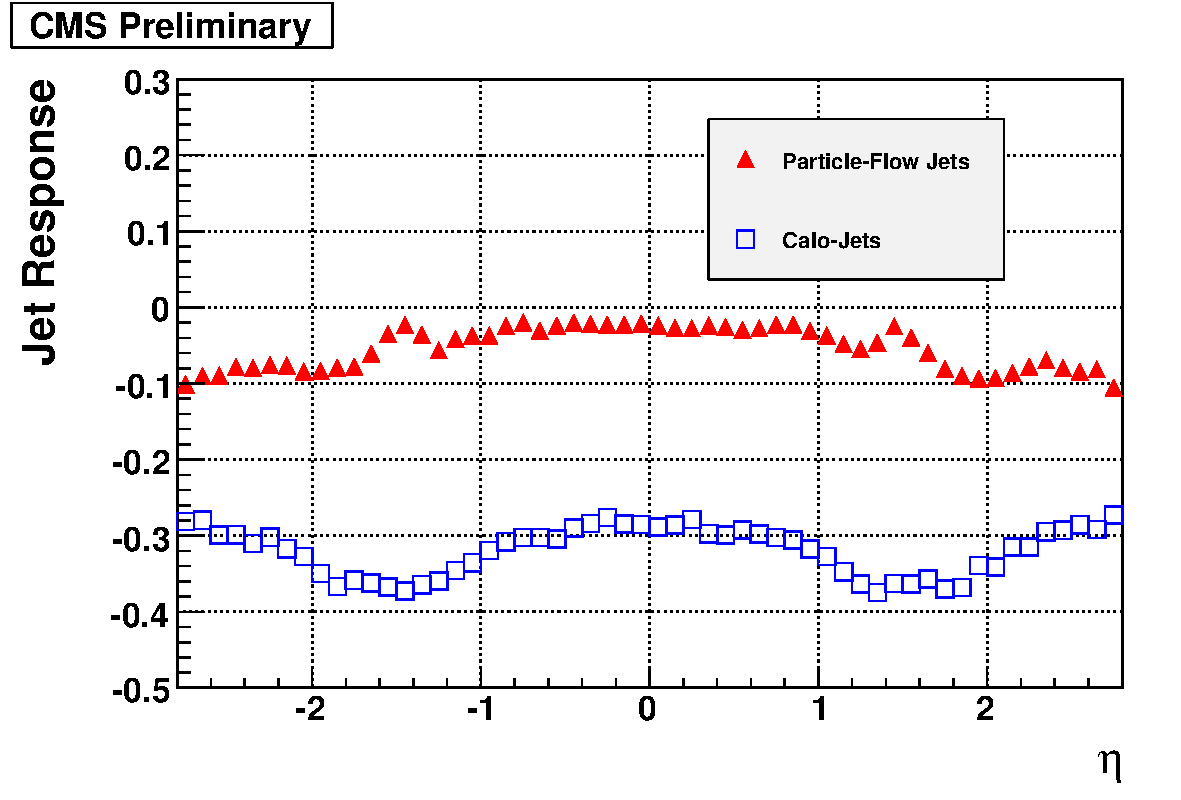
\includegraphics[width=0.79\textwidth]{Reconstruction/Figure_008-a-rotated90.pdf}\\
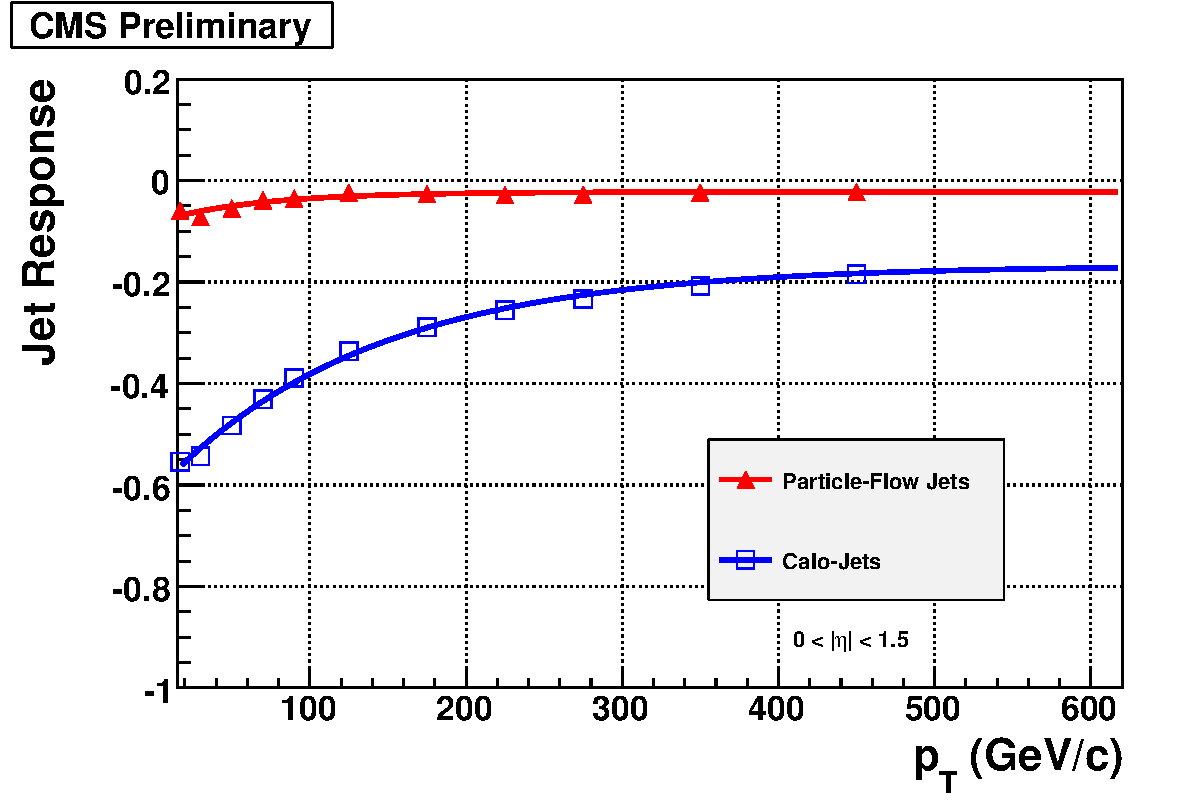
\includegraphics[width=0.49\textwidth]{Reconstruction/Figure_008-b-rotated90.pdf}
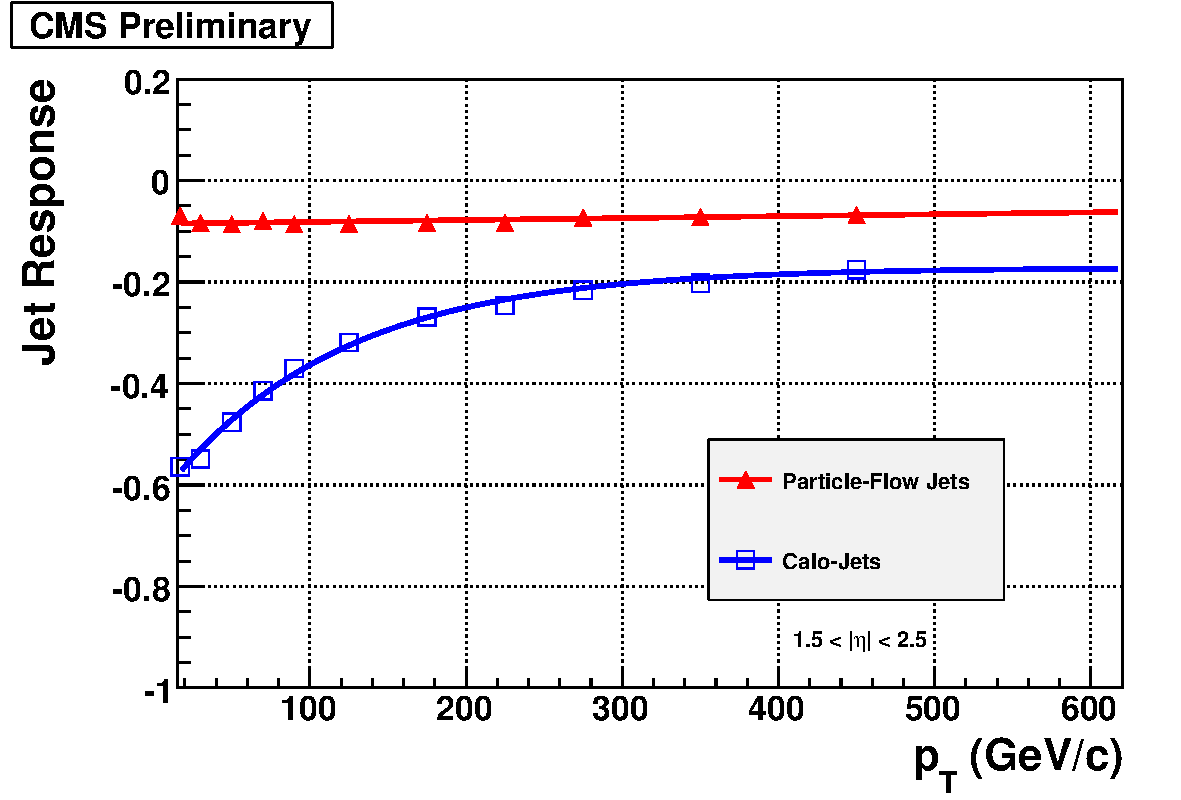
\includegraphics[width=0.49\textwidth]{Reconstruction/Figure_008-c-rotated90.pdf}
\caption{Jet response as a function of $\eta$ integrated over all $p_T$'s below 750 GeV (top) and as a function of $p_T$, in the barrel (left) and in the end-caps (right). The response curves are fit with exponential functions of $p_T$.~\cite{particleflow}}
\label{fig:jet_response}
\end{center}
\end{figure}


\begin{figure}
\begin{center}
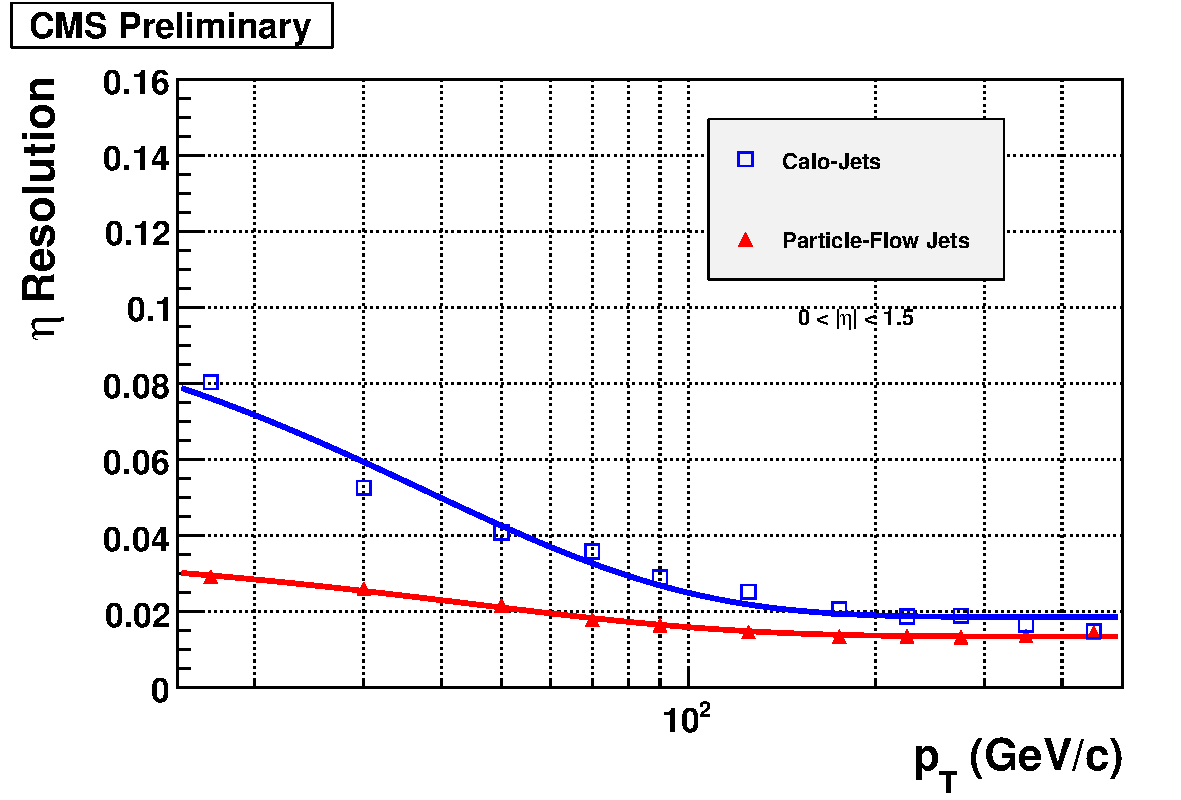
\includegraphics[width=0.49\textwidth]{Reconstruction/Figure_009-a-rotated90.pdf}
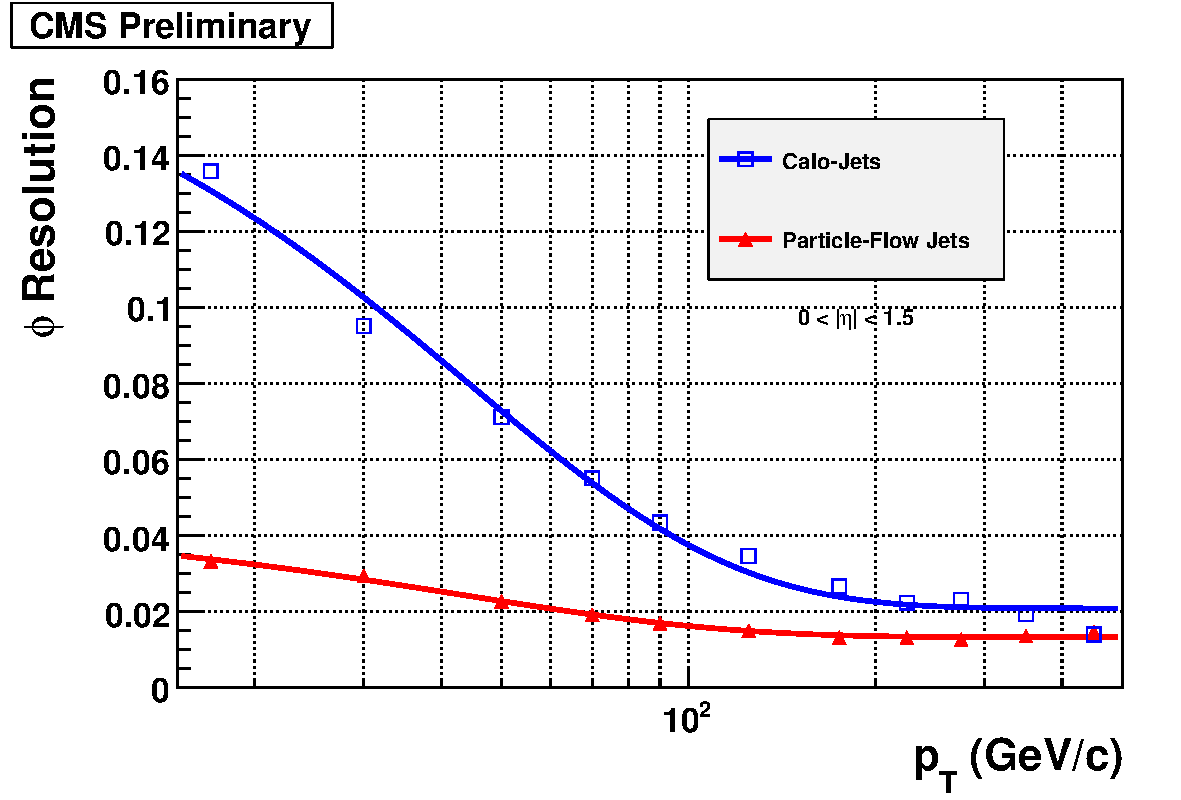
\includegraphics[width=0.49\textwidth]{Reconstruction/Figure_009-b-rotated90.pdf}
\caption{Jet-energy resolutions as a function of $p_T$ for corrected calo-jets and for particle-flow jets (upwards triangles) in the barrel (left) and in the end-caps (right). The resolution curves are fit to the sum of a constant term, a stochastic term and a noise term.~\cite{particleflow}}
\label{fig:jet_response_pt}
\end{center}
\end{figure}



%Pandolfi_jetenergy.pdf
